\section{Multi Configuration SCF}

The Hartree-Fock method is efficient when applied to closed-shell systems at
the equilibrium geometry. When these conditions are not met, the limited
flexibility of the wavefunction is not sufficient to describe the system.
The result is an incorrect representation of those electronic situations
which intrinsically need more than one determinant, and a wrong description
of the electron-electron repulsion effects.  The evaluation of the resulting
error, named \textit{correlation energy}, is central in any post-SCF
evaluation.

As already stated, the best solution is to consider the Full-CI expansion,
but practical computational factors limit this strategy to small molecular
systems. An intermediate solution is to pick a limited selection of
determinants, chosen under a given criterium. This approach
is generally called Multi Configuration or Multi Reference Configuration
Interaction (MRCI). 
A multireference approach provides additional flexibility to the
wavefunction, which can be used to describe those cases where the 
single-determinant Hartree-Fock approximation does not suffice, namely
geometrical distortion, bond breaking, or excited states.

\subsection*{A simple case: the hydrogen molecule}

The hydrogen molecule is the most frequently reported case to explain
problems related to a single-configuration approximation.
The molecular orbitals can be written as a linear combination of
$1s$ atomic orbitals (Linear Combination of Atomic Orbitals, LCAO),
normalized with a constant factor $N_1$:
\beq
\varphi_1=N_1 \left(1s_a + 1s_b \right)
\eeq
The resulting spatial orbital is doubly occupied, and the Slater determinant
is
\beq
\Phi_1 = \varphi_1(1) \varphi_1(2) \frac{\alpha \beta - \beta \alpha}{\sqrt{2}}
\eeq
where the spatial part $\varphi$ and the spin part have been separated for
the singlet closed-shell system.  Using this wavefunction to describe the
equilibrium geometry, the obtained results match qualitatively the
experimental values.

Developing the product for $ \Phi_1 $
\beqa
\Phi_1 &=& N_1^2 \left( 1s_a (1) + 1s_b (1)\right) \left( 1s_a (2) + 1s_b (2)\right) \mathcal{S}_0 (s_1,s_2) \nonumber \\
&=& N_1^2 \left[ \left( 1s_a (1) 1s_a (2) + 1s_b (1) 1s_b (2) \right) \right. \nonumber \\
& & + \left. \left( 1s_a (1) 1s_b (2) +  1s_b (1) 1s_a (2) \right) \right] \mathcal{S}_0 (s_1,s_2)
\eeqa
where $\mathcal{S}_0 (s_1, s_2) = \frac{\alpha \beta - \beta \alpha}{\sqrt{2}}$.
It is possible to recognize a ionic component (two electrons belong to the
same atom) and a covalent one (two equally shared electrons).
The single determinant expansion gives the same weight to these
representations, regardless of the interatomic distance. Rather obviously,
this interpretation does not hold when the molecule is completely
dissociated, and the ionic component with both electrons on the same atom is
supposed to be zero due to the high distance. As a resulting consequence,
the resulting SCF energy behaves incorrectly (Fig. \ref{fig:hydrogen})

If we build a two determinant MRCI
\beq
\Psi_{\mbox{\tiny MRCI}} = c_1 \Phi_1 + c_2 \Phi_2
\eeq
where $\Phi_2$ is the antibonding configuration
\beq
\Phi_2 = \varphi_2(1) \varphi_2(2) \frac{\alpha \beta - \beta \alpha}{\sqrt{2}}
\eeq
made with the difference
\beq
\varphi_2=N_2 \left( 1s_a - 1s_b \right)
\eeq
the resulting wavefunction can be optimized with additional degrees of
freedom, which provide a way for balancing the ionic and covalent components
with respect to the interatomic distance. This function shows the correct
dissociation curve.

\begin{center}
\begin{figure}[ht]
\begin{center}
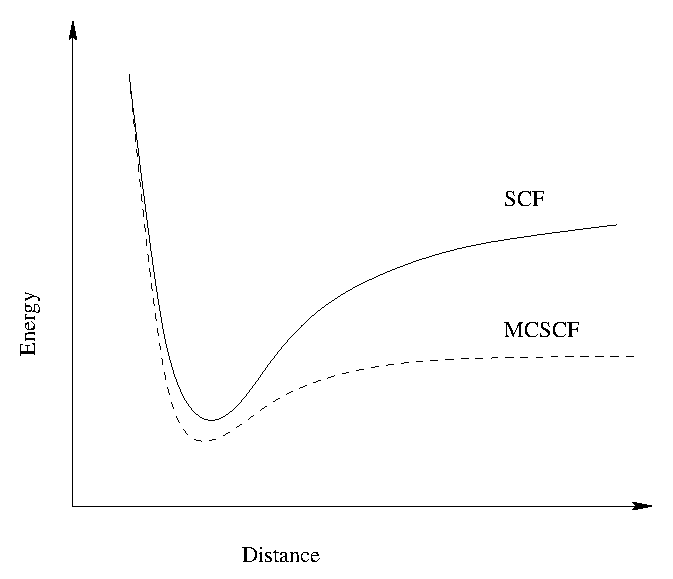
\includegraphics[width=11cm]{01_introduction/images/hydrogen.eps}
\end{center}
\caption{\footnotesize A qualitative behavior for the dissociation of the hydrogen
molecule.}
\label{fig:hydrogen}
\end{figure}
\end{center}


\subsection*{Complete Active Space}

The Complete Active Space (CAS) multiconfiguration selection is based on
the classification of the orbitals in three distinct groups: 
\textit{virtual orbitals}, always empty in each determinant of the CI
expansion, \textit{active orbitals} occupied in all the possible
configurations by a given number of \textit{active electrons}, and
\textit{core orbitals}, always occupied by electrons in each determinant of
the CI expansion.

This approach resembles a Full-CI limited to the set of active orbitals, 
and reduces the computational cost without renouncing too much on
wavefunction flexibility. The current limit for this technique is
14 active orbitals distributed in 14 electrons. Higher selections are
difficult to evaluate without dedicated algorithms, due to the high
computational cost involved in the operation.

\subsection*{Newton-Raphson algorithm}

To obtain an optimized multireference wavefunction, an optimization strategy
is needed. The Newton-Raphson method is one of these strategies. In this
algorithm, the energy $E$ is considered as a function of a set of
parameters, arranged as a vector $\mathbf{p}$. The function is then
expressed as a Taylor's expansion around a point $\mathbf{p}_0$
\beq
E(\mathbf{p}) = E(\mathbf{p}_0) + \sumidx{i} \left( \frac{\partial E}{\partial
p_i}\right)_{\mathbf{p}_0} p_i + \half \sumidx{i,j} p_i \left( \frac{\partial^2 E}{\partial
p_i \partial p_j} \right)_{\mathbf{p}_0} p_j + \ldots
\eeq
In matrix notation
\beq
E(\mathbf{p}) = E(\mathbf{p}_0) + \mathbf{g}^+\mathbf{p} + \half
\mathbf{p}^+\mathbf{H}\mathbf{p} + \ldots
\eeq
where $\mathbf{g}$ is the \textit{energy gradient vector} and 
$\mathbf{H}$ is the \textit{energy Hessian matrix}.
When evaluated in an energy minimum, the gradient vector is zero. An
iterative procedure exists, which involves the resolution of the linear
equation
\beq
\mathbf{g} + \mathbf{Hp} = \mathbf{0} 
\eeq
then redefining a new zero point from the obtained solution, evaluating
again $\mathbf{g}$ and $\mathbf{H}$ and stepping toward the solution. The
procedure is not guaranteed to converge to a minimum: in some cases it can
converge to saddle points or even diverge if the guess vector is too far
from the solution.

\subsection*{Super-CI method}

An alternative method is the Super-CI approach, which is based on the
extended version of the Brillouin theorem.  This theorem states that the
interaction between an optimized multireference wavefunction and its single
contracted excitations is zero.\cite{ijqc-2-307-1968} The optimization procedure
aims at nullifying iteratively these interactions to produce the optimized
solution.

A Super-CI wavefunction is built as
\beq
\ket{\mbox{SCI}} = \ket{\Psi_{0}} + \sumidx{p>q}t_{pq}E_{pq}^-\ket{\Psi_{0}}
\eeq
where $E_{pq}^- = E_{pq} - E_{qp}$ and $\ket{\Psi_{0}}$ is a multireference
wavefunction. The $E_{pq}$ operator is called \textit{shift operator} and is
useful to work with spatial orbitals, regardless of spin. It is expressed as 
\beq
E_{pq} = \constr{p \alpha } \destr{q \alpha} + \constr{p \beta}\destr{q
\beta}
\eeq
The convergence is reached when 
\beq
\braket{\Psi_{0}}{\ham}{E_{pq}^- \Psi_{0}} = 0
\eeq
We must note that single excitations are not orthonormal
\beqa 
S_{pq,rs} &=& \integral{E_{pq}^- \Psi_{0}}{E_{rs}^- \Psi_{0}} \\
&=& \braket{\Psi_{0}}{E_{qp}^-E_{rs}^-}{\Psi_{0}} \\
& \neq & \delta_{pq,rs}
\eeqa
The Hamiltonian matrix elements are
\beqa 
\braket{\Psi_{0}}{\ham}{pq} &=& \braket{\Psi_{0}}{\ham E_{pq}^-}{\Psi_{0}} = w_{pq} \\
\braket{pq}{\ham}{rs} &=& \braket{\Psi_{0}}{E_{qp}^-\ham E_{rs}^-}{\Psi_{0}} = d_{pq,rs}
\eeqa
and the secular equation to solve is
\beq
\left(
\begin{array}{cc}
E_{0} & \mathbf{w}^+ \\
\mathbf{w} & \mathbf{d}
\end{array} \right)
\left(
\begin{array}{c}
1 \\
\mathbf{t} \\
\end{array}
\right)
= E_{\mbox{\tiny SCI}}
\left(
\begin{array}{cc}
1 & \mathbf{0} \\
\mathbf{0} & \mathbf{S}
\end{array}
\right)
\left(
\begin{array}{c}
1 \\
\mathbf{t} \\
\end{array}
\right)
\eeq
which can be rewritten as
\beq
\left(
\begin{array}{cc}
0 & \mathbf{w}^+ \\
\mathbf{w} & \mathbf{d}-E_{0}\mathbf{S}
\end{array} \right)
\left(
\begin{array}{c}
1 \\
\mathbf{t} \\
\end{array}
\right)
= \left( E_{\mbox{\tiny SCI}} - E_{0} \right)
\left(
\begin{array}{cc}
1 & \mathbf{0} \\
\mathbf{0} & \mathbf{S}
\end{array}
\right)
\left(
\begin{array}{c}
1 \\
\mathbf{t} \\
\end{array}
\right)
\eeq

The Super-CI method is guaranteed to converge to a minimum, in
contrast to the Newton-Raphson method.

